\chapter{Grundlagen}
\section{Grundbegriffe}

\textbf{Big Data}\vspace{0.2cm}

Eine Abgrenzung des Begriff Big Data ist nicht eindeutig, da der Begriff sehr heterogen verwendet wird. Somit gibt es viele Definitionen vom Begriff Big Data.\vspace{0.2cm}

Als Big Data werden Daten bezeichnet, die entweder zu groß, zu komplex, zu schnelllebig oder zu schwach strukturiert sind, um diese mit herkömmlichen Methoden auszuwerten. Big bezieht sich in der Definition auf die vier Dimensionen. In Big Data sind Technologien die richtigen Informationen dem richtigen Adressaten zur richtigen Zeit in der richtigen Menge am richtigen Ort und in der erforderlichen Qualität bereitstellen.\vspace{0.2cm}

Auch strukturierte Daten. Verschiedene (autonome) Datenquellen (Datenbanken oder Anwendungen).\vspace{0.2cm}

Auf volume (Umfang, Datenvolumen), velocity (Geschwindigkeit, mit der die Datenmengen generiert und transferiert werden), variety (Bandbreite der Datentypen und -quellen) und veracity (Echtheit von Daten).\vspace{0.5cm}

\textbf{Knowledge Discovery in Data (-base)}\vspace{0.2cm}

Dies hat das Ziel aus vorhandenen meist großen Datenbeständen, fachliche Zusammenhänge zu erkennen. Zu den Teilschritten des KDD Prozesses gehören 1. Bereitstellung von Hintergrundwissen, 2. Definition der Ziele, 3. Datenauswahl, 4. Datenbereinigung, 5. Datenreduktion, 6 Auswahl eines Modells, 7. Data-Mining, die eigentliche Datenanalyse, 8. Interpretation der gewonnenen Erkenntnisse.\vspace{0.5cm}

\textbf{Data-Mining}\vspace{0.2cm}

Data-Mining die systematische Anwendung von statischen Methoden auf große Datenbestände, um neue Querverbindungen zu erkennen. Data-Mining ist ein Teilprozess KDD Prozesses. Mit Data-Mining findet ein Informationsgewinn oder -erweiterung, aus den Big Data statt. Hier werden Algorithmen aus dem Bereich ML angewandt.

k-Means Algorithmus\vspace{0.5cm}

\textbf{Machine Learning}\vspace{0.2cm}

Maschinelles Lernen (eng. Machine Learning) ist nach [https://datasolut.com/was-ist-machine-learning] ein Teilbereich der künstlichen Intelligenz, der System in die Lage versetzt, automatisch aus Erfahrungen (Daten) zu lernen und sich zu verbessern. Aufgaben die Machine Learning erledigen kann, ist Berechnung von Wahrscheinlichkeiten für bestimmte Ereignisse, Erkennen von Gruppen und Clustern in Datensätzen, Erkennen von Zusammenhängen in Sequenzen, Reduktion von Dimensionen ohne großen Informationsverlust und Optimierung von Geschäftsprozessen.\vspace{0.5cm}

\textbf{Künstliche Intelligenz}\vspace{0.2cm}

Eine einheitliche gemeingültige Definition von künstlicher Intelligenz zu geben ist nicht einfach. Zuvor muss Intelligenz definiert werden. Aber was ist Intelligenz? In der Literatur werden kognitive Fähigkeiten oft mit Intelligenz in Verbindung gebracht.
In der Definition von künstlicher Intelligenz gibt es schwache oder enge künstliche Intelligenz, die auf die Lösung bestimmter Aufgaben beschränkt ist und menschliche Intelligenz nicht imitieren kann. Starke oder allgemeine künstliche Intelligenz hingegen ist in der Lage die kognitiven Fähigkeiten des Menschen zu erzielen.\vspace{0.5cm}

Weitere Definitionen werden im Verlauf der Arbeit ergänzt.

\section{Verwandte Arbeiten}
Mit weiteren Anwendungsfällen beschäftigt sich das ,,Fraunhofer Institut BIG DATA'' in ihrem Paper [\href{https://www.bigdata-ai.fraunhofer.de/content/dam/bigdata/de/documents/Publikationen/KI-Potenzialanalyse_2017.pdf}{Big Data Frauenhofer}].\vspace{0.2cm}

Um den Einsatz künstlicher Intelligenz im werte-orientierten Marketing zu bewerten, befassten sich in [\href{https://www.econstor.eu/bitstream/10419/222610/1/1725938928.pdf}{EConster}] einige Professoren des ,,Leibniz-Informationszentrum Wirtschaft'' mit diesem Thema.\vspace{0.2cm}

Die Masterarbeit [\href{https://reposit.haw-hamburg.de/bitstream/20.500.12738/7932/1/master_thesis.pdf}{Bitstream}] von Eduard Weigandt befasst sich mit der Personalisierung im E-Commerce basierend auf Data-Mining. Interessante Grundlagen zum Einstieg in E-Commerce und künstlicher Intelligenz sind auf [\href{https://www.epoq.de/blog}{Eqop}] zu finden. Die Firma Kobold AI befasst sich in ihrem Artikel [\href{https://www.kobold.ai/kundensegmentierung-ki}{Kobold.ai}] ,,Optimale Segmentierung von Bestandskunden durch KI'' und erläutert Methoden zur Clustering von Bestandskunden. ,,Datasolut'' ist ein weiteres Unternehmen das sich in [\href{https://datasolut.com/kundenklassifizierung-definition-vorteile-und-methoden}{Datasolut1}] mit Kundenklassifizierung, Clusteranalyse und maschinellem Lernen befasst. Ebenfalls von ,,Datasolut'' ist der Artikel [\href{https://datasolut.com/ki-im-e-commerce}{Datasolut2}] in dem erfolgreiche Anwendungen und Beispiele zum Thema künstlicher Intelligenz im E-Commerce aufgezeigt werden.

\section{Big Data}
Big Data beschäftigt sich nach [\href{https://datasolut.com/was-ist-big-data}{DataSolut3}] und [\href{https://www.oracle.com/de/big-data/what-is-big-data}{Oracle}] mit dem Sammeln, Verarbeiten und Zusammenführen von großen Datenmengen. Um diese Daten für die Entscheidungsfindung und Prozessautomatisierung zu verwenden. Dabei stammen die Daten aus den unterschiedlichsten Quellen, aus verschiedenen Datenbanken oder auch direkt aus Programmen. Als Datenquellen können folgende infrage kommen:

\begin{itemize}
	\item Internetnutzung
	\item Social Media
	\item Geo-Tracking
	\item Cloud Computing
	\item Vitaldaten-Messung
	\item Media-Streaming
\end{itemize}

Diese Daten können strukturiert, aber auch unstrukturiert vorliegen. [Gratner] beschrieb Big Data anhand von den ,,4 V's''. Mit der Zeit wurde es um ein ,,V'' erweitert. Diese Beschreibung wird in unterschiedlichen Publikationen aufgegriffen, unter anderen auch in [\href{https://www.oracle.com/de/big-data/what-is-big-data}{Oracle}].\vspace{0.5cm}

\textbf{Volume (Volumen)}\vspace{0.2cm}

Immer größere Datenmengen müssen Verarbeitet werden. Durch die stetig zunehmende Digitalisierung in immer mehr Lebensbereichen wächst die erzeugte Datenmenge pro Zeiteinheit immer mehr an. So werden großen Datenmengen nicht nur durch die oben genannten Quellen erzeugt, sondern auch z. B. durch Gerätesensoren. Hierbei können etliche Terabytes oder hunderte Petabytes an Daten anfallen. Wie die Abbildung \ref{img:stat_prognose_2022} [\href{https://de.statista.com/statistik/daten/studie/267974/umfrage/prognose-zum-weltweit-generierten-datenvolumen}{Statistika}] zeigt, wird das Datenvolumen im Jahr 2025 auf 181 Zettabyte vorhergesagt.\vspace{0.2cm}

\begin{figure}[!ht]
	\centering
	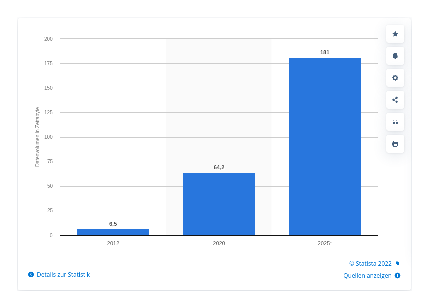
\includegraphics[width=\linewidth]{images/chapter2/umsatzprognose_2025.eps}
	\caption{Umsatzprognose E-Commerce bis 2025}
	\label{img:stat_prognose_2022}
\end{figure}


\textbf{Variety (Vielfalt)}\vspace{0.2cm}

Durch die unterschiedlichen Bereiche, in denen die Datenmengen entstehen sind, diese sehr unterschiedlich und zu meist unstrukturiert. Oft liegen diese in relationalen Datenbanken und können dort nicht ausgewertet werden. Neben Texten liegen die Daten in Bildern und Videos vor die Analyse erfolgt durch Machine Learning Algorithmen .\vspace{0.5cm}

\textbf{Velocity (Geschwindigkeit)}\vspace{0.2cm}

Mit der Entwicklung der Technik produzieren Softwaresysteme mit einer höheren Geschwindigkeit mehr Daten. Bei vielen Produkten fließen die Daten nicht auf eine Festplatte, sondern werden direkt im Speicher verarbeitet. Solche Produkte arbeiten in Echzeit oder beinahe in Echtzeit. Deren Verarbeitung in immer kürzerer Zeit erfolgt. Für Unternehmen und verschiedenen Use Cases kann die Verarbeitung in Echtzeit einen erheblichen Wettbewerbsvorteil bedeuten.\vspace{0.5cm}

\textbf{Veracity (Wahrhaftigkeit)}\vspace{0.2cm}

Da die Daten oft aus Quellen kommen, deren Wahrheitsgehalt nicht sicher ist und die Daten in nicht geeigneter Qualität vorliegen, können diese nicht ohne eine aufwendige Nachbearbeitung eingesetzt werden.\vspace{0.5cm}

\textbf{Value (Mehrwert)}\vspace{0.2cm}

Durch die Verknüpfung der Daten, die beim Einsatz der Techniken des Machine Learning entstehen, ist dieser Mehrwert eines der wichtigsten ,,V'' bei Big Data. Ohne diesen Mehrwert würde Big Data keinen Sinn ergeben.

\subsection{Technologien}
Rund um das Thema Big Data, haben sich verschiedene Technologien entwickelt, die Ansätze für die Verarbeitung von großen Datenmengen liefern. Nachfolgende sind Open Source Produkte stellvertretend einige genannt.\vspace{0.2cm}

\textbf{Apache Spark}\vspace{0.2cm}

Es ist nach eigenen Angaben [\href{https://spark.apache.org}{Spark}] eine mehrsprachige Engine zur Ausführung von Data Engineering, Data Science und maschinelles Lernen auf Single-Node-Maschinen oder Clustern.\vspace{0.5cm}

\textbf{Apache Hadoop}\vspace{0.2cm}

Hadoop ist nach [\href{https://hadoop.apache.org}{Hadoop}] ein Framework das mit einfachen Programmiermodellen, welches eine verteilte Verarbeitung von großen Datenmengen anbietet, das von einzelnen Server auf mehrere tausend skaliert werden kann.\vspace{0.5cm}

\textbf{Apache Cassandra}\vspace{0.2cm}

Nach eigener Beschreibung [\href{https://cassandra.apache.org}{Cassandra}], ist Cassandra ist ein skalierbares und hochverfügbares verteiltes Datenbanksystem. Es basiert auf NoSQL, ist Open-Source und kann ebenfalls auf einzelnen Servern oder in der Cloud eingesetzt werden.

\section{Data-Mining}
\section{Clustering}


Abkürzungen\\
ML Mashine Learning\\
KI Künstliche Intelligenz